\documentclass[12pt, a4paper]{article}
\usepackage[margin=15mm]{geometry}
\usepackage{tikz}
\usetikzlibrary{3d,calc}

\begin{document}

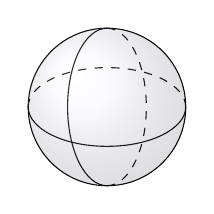
\begin{tikzpicture}
    \draw (-1,0) arc (180:360:1cm and 0.5cm);
    \draw[dashed] (-1,0) arc (180:0:1cm and 0.5cm);
    \draw (0,1) arc (90:270:0.5cm and 1cm);
    \draw[dashed] (0,1) arc (90:-90:0.5cm and 1cm);
    \draw (0,0) circle (1cm);
    \shade[ball color=blue!10!white,opacity=0.20] (0,0) circle (1cm);
\end{tikzpicture}

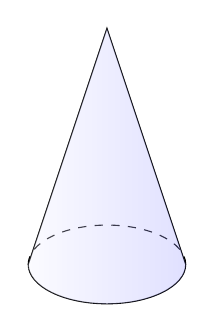
\begin{tikzpicture}
    \draw (-1,0) arc (180:360:1cm and 0.5cm) -- (0,3) -- cycle;
    \draw[dashed] (-1,0) arc (180:0:1cm and 0.5cm);
    \shade[left color=blue!5!white,right color=blue!40!white,opacity=0.3] (-1,0) arc (180:360:1cm and 0.5cm) -- (0,3) -- cycle;
\end{tikzpicture}

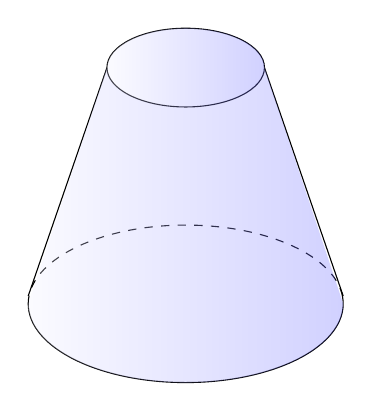
\begin{tikzpicture}
    \draw (-1,0) arc (180:360:1cm and 0.5cm);
    \draw (-1,0) arc (180:0:1cm and 0.5cm);
    \draw (-2,-3) arc (180:370:2cm and 1cm);
    \draw[dashed] (-2,-3) arc (180:10:2cm and 1cm);
    \draw(-2,-2.9)  -- (-1,0);
    \draw(2,-2.9)   -- (1,0);
    \shade[left color=blue!5!white,right color=blue!60!white,opacity=0.3] (-1,0) arc (180:360:1cm and 0.5cm) -- (2,-3) arc (360:180:2cm and 1cm) -- cycle;
    \shade[left color=blue!5!white,right color=blue!60!white,opacity=0.3] (0,0) circle (1cm and 0.5cm);
\end{tikzpicture}

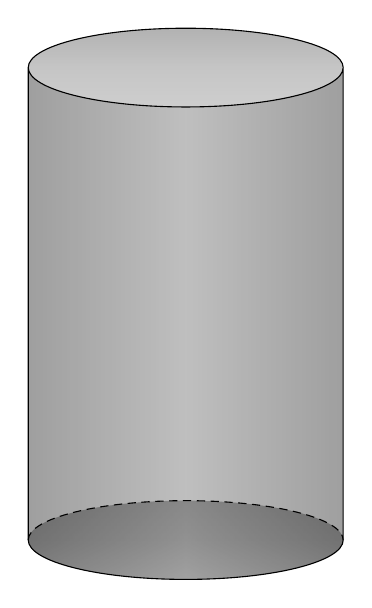
\begin{tikzpicture}
	\fill[top color=gray!50!black,bottom color=gray!10,middle color=gray,shading=axis,opacity=0.25] (0,0) circle (2cm and 0.5cm);
	\fill[left color=gray!50!black,right color=gray!50!black,middle color=gray!50,shading=axis,opacity=0.25] (2,0) -- (2,6) arc (360:180:2cm and 0.5cm) -- (-2,0) arc (180:360:2cm and 0.5cm);
	\fill[top color=gray!90!,bottom color=gray!2,middle color=gray!30,shading=axis,opacity=0.25] (0,6) circle (2cm and 0.5cm);
	\draw (-2,6) -- (-2,0) arc (180:360:2cm and 0.5cm) -- (2,6) ++ (-2,0) circle (2cm and 0.5cm);
	\draw[densely dashed] (-2,0) arc (180:0:2cm and 0.5cm);
\end{tikzpicture}

\end{document}